%!TEX root = proj_report_outline.tex

\chapter{Web Application Design}
The design of the web application focused on the use of standard architecture patterns and web development technologies. This approach was taken as web application development covers numerous domains and technologies. In \citeauthor{shklar2009web}'s tome ``Web Application Architecture: Principles, Protocols and Practices'' they describe the core areas of knowledge required: HTTP, HTML, SMTP, JavaScript, Databases, Graphics Design, and Server Technology \cite{shklar2009web}. While designing a unique foundation specifically optimised for PitchHub is enticing, as Donald Knuth is famously quoted ``97\% of the time premature optimization is the root of all evil'' \cite{knuth1974structured}. Furthermore, given the time constraints of this project, PitchHub leverages battle tested open source libraries to deliver more functionality while reserving the ability to make custom modifications and changes as necessary. This chapter explores these design choices and also the alternative designs that were considered throughout this project.

\section{Architecture}

The architecture of the web application was the first work accomplished on PitchHub. The architecture is the abstraction of the system and hence should be designed with the desired system qualities needed to to be achieved. With PitchHub the security and distributed requirements identified in Chapter \ref{C:requirements} were captured in the three tier architecture designed, hence formalising the requirements specification early on.
\par
The common software engineering practice of separation of concerns has a strong presence within this architecture as seen in Figure \ref{fig:architecture_1}. Each tier's logic and responsibilities is encapsulated from the other tiers. Their only knowledge of the outside world is in the design-time defined interfaces of their neighbouring tiers. To partially fulfil the security requirement PitchHub communicates using the \textit{Transport Layer Security} (TLS) protocol, that provides secure bidirectional communication between the client and server.
\par
The data layer is designed in a distributed configuration where database nodes may be scaled horizontally. There are a variety of reasons why this is important to PitchHub. The data intensive nature of PitchHub means that it can improve it's performance through spreading the data and processing logic among nodes. This kind of approach is known as a shared nothing architecture \cite{stonebraker1986case}, prevalent in NoSQL systems.
\par
In Figure \ref{fig:architecture_1} within the Client and Server layers the Model-View-Controller architecture pattern has been employed continuing the design theme of separation of concerns. To unpack this term: models maintain state, usually communicating with a database, controllers coordinate interaction and are responsible for delegating tasks to models and views determine what data is rendered from the model. This separation of responsibilities enables complex sets of interactions to be standardised, conforming to conventions that are well defined and that can be easily be understood \cite{leff2001web}.

\begin{figure}[ht]
    \centering
    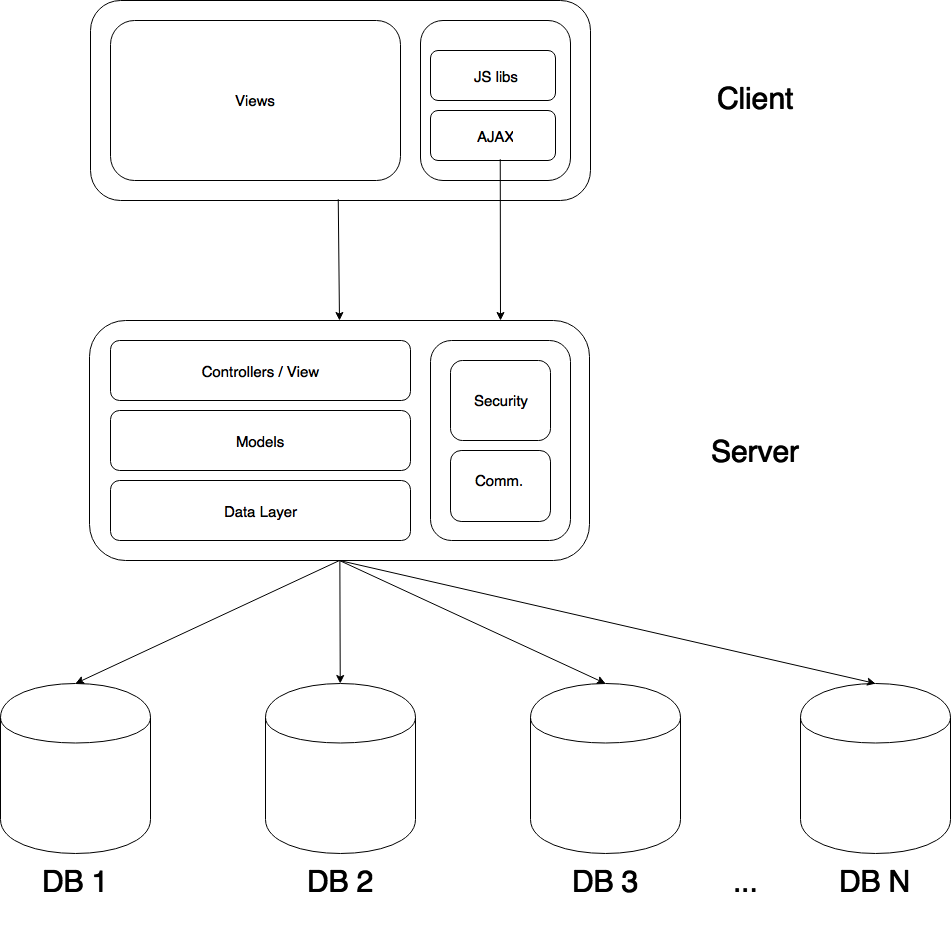
\includegraphics[width=1\textwidth]{architecture_1}
    \caption{The 3-tier architecture used in PitchHub capturing the security and distributed requirements identified in Chapter \ref{C:requirements} in the design.}
    \label{fig:architecture_1}
\end{figure}

\section{System Model}

The design of the system's model is another case of requirements being captured early in the design phase. Figure \ref{fig:class_diagram} illustrates the system's classes and their relationships as a class diagram. The requirement to implement privacy controls is captured in the Pitch Card and Comment classes' relationship with the DisclosureScope class. To illustrate this it is important to understand how the platform works: A user creates a Pitch Card, detailing the idea's attributes in the Pitch Card's Pitch Points, their aim is to get the community to collaborate on the Pitch Card to derive meaningful information or connections to action the Pitch Card, collaborator's on a Pitch Card can make suggestions or comments on these Pitch Points to help drive the idea forward. By providing scoping on Pitch Cards initiator's set a base restriction level for the Pitch Card and it's related content. The negotiation aspect of PitchHub is introduced with the Comments and Suggestions users may contribute to PitchCards. As seen in Figure \ref{fig:class_diagram} these classes also have scoping, however in this case scoping can only be set to an equivalent or more restrictive level than that specified in the Pitch Card. An example of this is where an initiator set's the content scope to `Members', so only members of the PitchHub can view the idea, now if a user were to contribute a suggestion on a Pitch Point this suggestion can only be scoped as `Members' or any level which is more restrictive, they cannot however set it to `Public'. This interaction/requirement as seen in Figure \ref{fig:class_diagram} is designed with the Strategy Pattern so that future scopes will have minimal change to the application.
 
\begin{sidewaysfigure}[ht]
    \centering
    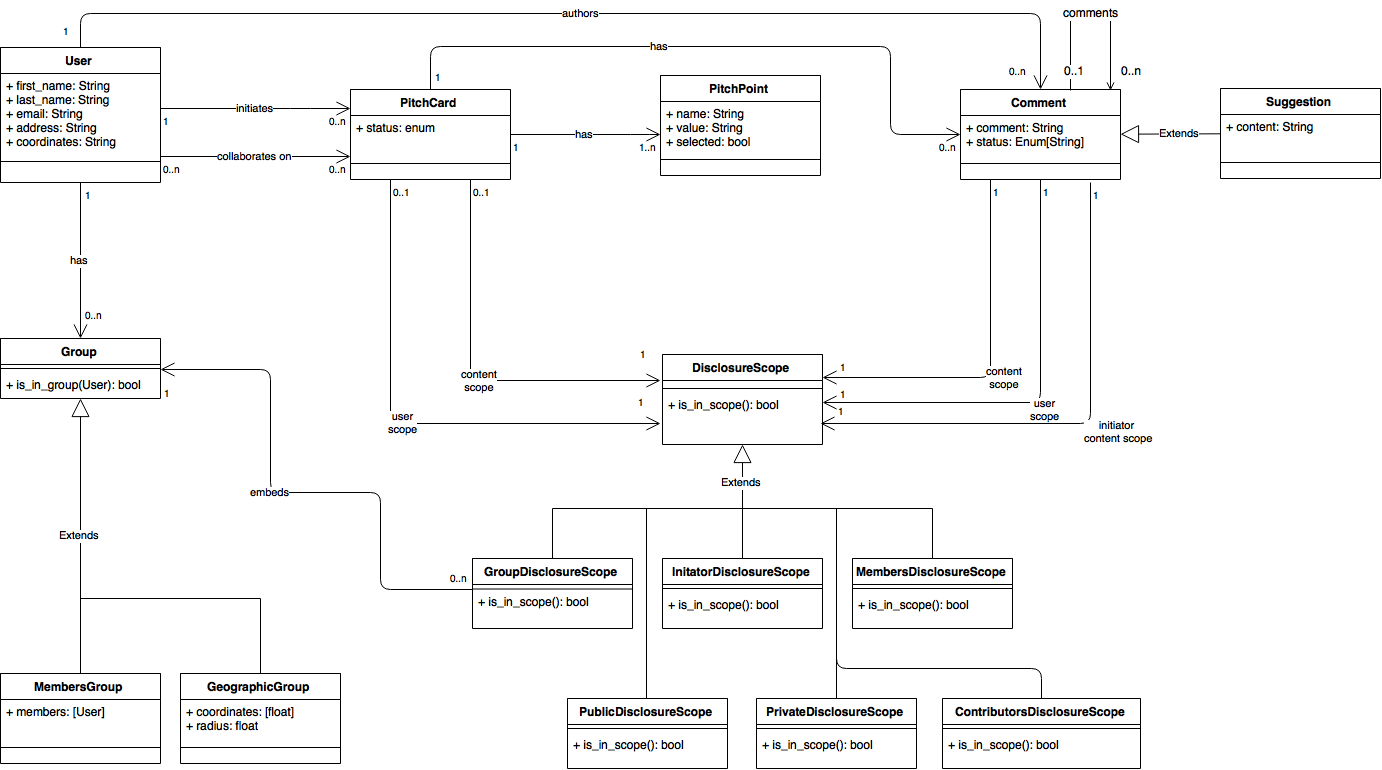
\includegraphics[width=1\textwidth]{class_diagram}
    \caption{PitchHub's system structure as represented in a class diagram. Of note is the Pitch Card and Comment classes and their relationship to the DisclosureScopes. This relationship describes the Pitch Card and Comment classes ability to scope the visibility of their content. (NB: Some attributes were left out for the sake of brevity e.g. Pitch Cards have an `images' attribute)}
    \label{fig:class_diagram}
\end{sidewaysfigure}

\section{Technology Choice}

The quality of service attributes of a web application are deeply influenced by the fundamental technologies backing the solution. In this section both the framework and database selections are discussed in relation to quality of service attributes and more importantly the requirements identified in Chapter \ref{C:requirements}.

\subsection{Framework Selection}

Research was conducted on the web application frameworks available in effort to speed up the prototyping process. Ruby on Rails, Laravel, Django, MEAN and OpenSocial were identified as frameworks that could work in fulfilment of the requirements specified. Ultimately the choice of frameworks was between Ruby on Rails and OpenSocial as they are written in languages that I most understand (Ruby and Java, respectively). Ruby on Rails is an open source framework that embraces RESTful web service design and conforms to the MVC architecture. Of note, Ruby on Rails has a wealth of open-source secret sharing and functional testing libraries that are directly applicable to the requirements of this project. OpenSocial in contrast to Ruby on Rails is first and foremost a framework for creating social network, and while PitchHub is not specifically a social network it's primary objective is to facilitate social interaction. Using OpenSocial would offer user authentication as well as messaging and posting functionality out of the box. 
\par
Of these frameworks Ruby on Rails was selected because of its vast open source library and elegant handling of complex user interaction flows. This decision results in a trade off in performance. Even in the current versions of each language Java has a significant  performance advantage over Ruby \cite{Perfo1:online}. For a simple web application this generally would not be a concern, however the secret sharing component entails the use of encryption algorithms which are computationally expensive. This was concluded not to be a major issue as Ruby on Rails offers the ability to run JRuby which is Ruby executed atop the JVM. JRuby offers significantly improved performance and even allows native Java to be executed if necessary \cite{Jruby:online}.

\subsection{Database Selection}

The choice of database has profound effects on the performance and scalability requirements identified in Chapter \ref{C:requirements}. The rise of NoSQL databases has been attributed to the increasing need for highly scalable and performant databases. Given this need in PitchHub, in addition to PostgreSQL, the NoSQL databases MongoDB and Cassandra were also investigated.
\par
The nature of the Pitch Card data PitchHub is modelling is inherently hierarchical and heterogeneous. In PitchHub, each Pitch Card has a varying number of Pitch Points, and each Pitch Point value also contains a number of interaction attributes. This data model naturally lends itself to the document model offered by MongoDB. Pitch Cards may be modelled in a single document with Pitch Point relations expressed via embedding. This has the additional benefit of being able to efficiently query this Pitch Cards.
\par
The case for using a relational database like PostgreSQL is also motivated by the inherent nature of PitchHub's data. For example, each user is associated to the Pitch Cards they have initiated and contributed to, as well as the suggestions and comments they have offered on Pitch Cards. Unlike the internal model of Pitch Cards these relations are not well suited to being hierarchical as these relations have associations which are N:M rather than 1:1 or 1:N. Modelling these objects separately in tables and querying them through joins in the relational model is the ideal way to represent and query these relations.
\par
Ultimately MongoDB was selected as the database for PitchHub. MongoDB was chosen because the Pitch Card data is well suited to this data and the use case flows which require joins at most only need one join operation. It was concluded that using MongoDB and performing manual joins within the application is not a major issue because of this. Also MongoDB's ability to scale horizontally easily without the expensive migrations characteristic of relational databases provides an edge over PostgreSQL in meeting the scalability requirement.

\section{Behaviour Driven Development}
The development of the web application in keeping with the iterative approach involved progress on many aspects of the project each week: requirements analysis, requirements validation, design, development, testing, and documentation.
Behaviour Driven Development (BDD) was incorporated within this process to ensure that the mutual understanding documented in the weekly reports was being directly (and accurately) translated into the prototype.
\par
This kind of development involved requirements being distilled into specifications, with the behaviour of the code being specified ahead of the implementation. This meant that the implementation then had the onus to fulfil the specified behaviour. With this approach PitchHub's progress was able to be tracked in each iteration in regards to actual business value being delivered. A by-product of this approach has resulted in PitchHub's test-suite relying less on tests on classes and units but on specification. The BDD process has been described as producing what is essentially executable documentation \cite{astels2006new}.
